%\documentclass[output=paper,modfonts,nonflat]{langscibook} 
%\bibliography{mwe2017bib3} 
%% add all extra packages you need to load to this file 
\usepackage{graphicx}
\usepackage{tabularx}
\usepackage{amsmath} 
\usepackage{multicol}
\usepackage{lipsum}
%%%%%%%%%%%%%%%%%%%%%%%%%%%%%%%%%%%%%%%%%%%%%%%%%%%%
%%%                                              %%%
%%%           Examples                           %%%
%%%                                              %%%
%%%%%%%%%%%%%%%%%%%%%%%%%%%%%%%%%%%%%%%%%%%%%%%%%%%%
% remove the percentage signs in the following lines
% if your book makes use of linguistic examples
\usepackage{langsci/styles/langsci-gb4e} 
\usepackage{langsci/styles/langsci-optional} 
\usepackage{langsci/styles/langsci-lgr}
\usepackage{langsci/styles/langsci-bidi}
\usepackage{morewrites} 
%% if you want the source line of examples to be in italics, uncomment the following line
% \def\exfont{\it}

%\usepackage{enumitem} %Conflict with enumerate
\usepackage{lipsum}
\usepackage{multirow}
\usepackage{graphicx}
\usepackage{epstopdf}
\usepackage{wrapfig}
\usepackage{caption}
\usepackage{subcaption}
\usepackage{url}
\usepackage{relsize}
\usepackage{paralist}
\usepackage{tabularx} 
%\newfontfamily\Parsifont[Script=Arabic]{langsci/fonts/ScheherazadeRegOT_Jazm.ttf} 
\usepackage{latexsym}
\usepackage{tikz-dependency}
\usepackage{textgreek}
\usepackage{color}
\usepackage{newfloat}
\usepackage{hhline}
\usepackage{xspace}
\usepackage{booktabs}
\usepackage{verbatim} 
\usepackage{algorithm}
\usepackage[noend]{algpseudocode}
\usepackage{sidecap}
\usepackage{kantlipsum}
\usepackage{verbatimbox} 
\usepackage[usestackEOL]{stackengine}
\usepackage{tikz}
\usetikzlibrary{shapes.arrows}
\usepackage{todonotes}
\usepackage{csquotes}
\usepackage{amsmath}
%\usepackage[british]{babel}
\usepackage{mathtools}  % better amsmath
\usepackage{dcolumn}
\newcolumntype{d}[0]{D{.}{.}{2}}
\usepackage{cjhebrew} % Hebrew
\usepackage[normalem]{ulem}
\usepackage{qtree}
\usepackage{rotating}
\usepackage[section]{placeins} 
\usepackage{soulutf8}  % \ul command for underlining
% \usepackage{langsci/styles/langsci-bidi}

\usepackage{booktabs} %Salehi et al.
\usepackage{makecell} %Bhatia


%%% hyphenation points for line breaks
%% Normally, automatic hyphenation in LaTeX is very good
%% If a word is mis-hyphenated, add it to this file
%%
%% add information to TeX file before \begin{document} with:
%% %% hyphenation points for line breaks
%% Normally, automatic hyphenation in LaTeX is very good
%% If a word is mis-hyphenated, add it to this file
%%
%% add information to TeX file before \begin{document} with:
%% %% hyphenation points for line breaks
%% Normally, automatic hyphenation in LaTeX is very good
%% If a word is mis-hyphenated, add it to this file
%%
%% add information to TeX file before \begin{document} with:
%% \include{localhyphenation}
\hyphenation{
affri-ca-te
affri-ca-tes
an-no-tated
com-ple-ments
com-po-si-tio-na-li-ty
non-com-po-si-tio-na-li-ty
Gon-zá-lez
out-side
Ri-chárd
se-man-tics
STREU-SLE
}
\hyphenation{
affri-ca-te
affri-ca-tes
an-no-tated
com-ple-ments
com-po-si-tio-na-li-ty
non-com-po-si-tio-na-li-ty
Gon-zá-lez
out-side
Ri-chárd
se-man-tics
STREU-SLE
}
\hyphenation{
affri-ca-te
affri-ca-tes
an-no-tated
com-ple-ments
com-po-si-tio-na-li-ty
non-com-po-si-tio-na-li-ty
Gon-zá-lez
out-side
Ri-chárd
se-man-tics
STREU-SLE
}
%%add all your local new commands to this file

\newcommand{\smiley}{:)}

\renewbibmacro*{index:name}[5]{%
  \usebibmacro{index:entry}{#1}
    {\iffieldundef{usera}{}{\thefield{usera}\actualoperator}\mkbibindexname{#2}{#3}{#4}{#5}}}

% \newcommand{\noop}[1]{}

%add all your local new commands to this file

\newcommand{\ie}{i.e., }

% \newcommand{\noop}[1]{}

\newcommand{\blex}[1]{\textit{#1}\xspace}

\newcommand{\ngram}[1][]{$n$-gram{#1}\xspace}

\newcommand{\mwetype}[1]{\texttt{#1}\xspace}
\newcommand{\strongish}{\mwetype{strong}}
\newcommand{\weak}{\mwetype{weak}}
%\newcommand{\hard}{\mwetype{hard}}
\newcommand{\hard}{\textit{hard}}
%\newcommand{\mixed}{\mwetype{mixed}}
\newcommand{\mixed}{\textit{mixed}}

\newcommand{\gap}{$*$\xspace}
\newcommand{\zp}{\phantom{0}}

\newcommand{\figureref}[1]{Figure~\ref{#1}\xspace}
\newcommand{\tableref}[1]{Table~\ref{#1}\xspace}
\newcommand{\sectionref}[1]{Section~\ref{#1}\xspace}


\DeclareFloatingEnvironment[fileext=lod]{diagram}
\newcommand{\nothing}[1]{}

\DeclareOldFontCommand{\bf}{\normalfont\bfseries}{\mathbf}
\DeclareOldFontCommand{\it}{\normalfont\bfseries}{\mathbf}
\DeclareOldFontCommand{\sc}{\normalfont\bfseries}{\mathbf}


% \newcommand{\noop}[1]{}


\newcommand{\class}[1]{\texttt{#1}\xspace}
\newcommand{\localex}[1]{\textit{#1}\xspace}
\newcommand{\gl}[1]{``{#1}''\xspace}

\newcommand{\x}{\phantom{0}}

% Style guide provides these...

\newcommand{\localtabref}[2][]{Table#1~\ref{#2}\xspace}
\newcommand{\secref}[2][]{Section#1~\ref{#2}\xspace}
\newcommand{\localfigref}[2][]{Figure#1~\ref{#2}\xspace}

\newcommand{\eqnref}[2][]{Equation#1~\ref{#2}\xspace}

\newcommand{\REDDY}{ENC\xspace}
\newcommand{\BANNARD}{EVPC\xspace}

\newcommand{\MWE}{\ensuremath{\mathit{mwe}}}
\newcommand{\component}{\ensuremath{\mathit{component}}}

\newcommand{\spadeaff}{\ensuremath{\spadesuit}\xspace}
\newcommand{\clubaff}{\ensuremath{\clubsuit}\xspace}
\newcommand{\heartaff}{\ensuremath{\heartsuit}\xspace}
\newcommand{\diamondaff}{\ensuremath{\diamondsuit}\xspace}


\newcommand{\CS}[1]{\ensuremath{\mathit{CS}_{\mathit{#1}}}\xspace}

\newcommand{\CSsource}{\CS{L1}}
\newcommand{\CStarg}{\CS{L2N}}
\newcommand{\CSsourcetarg}{\CS{L1+L2N}}
\newcommand{\CSsvr}{\CS{SVR(L1+L2)}}
\newcommand{\CSstring}{\CS{string}}
\newcommand{\CSall}{\CS{all}}
\newcommand{\CSstringDS}{\CS{string+L1}}

%add all your local new commands to this file

\newcommand{\main}[1]{\textbf{#1}}

%\newcommand{\dataset}[1]{\textsc{#1}\xspace}

%\newcommand{\dataset}[1]{\textsc{#1}}

\newcommand{\feat}[1]{{\textsc{#1}}}
\newcommand{\swfeat}[2]{\feat{#1$_{#2}$}}
\newcommand{\bgfeat}[3]{\feat{#1$_{#2}$#1$_{#3}$}}
\newcommand{\tgfeat}[4]{\feat{#1$_{#2}$#1$_{#3}$#1$_{#4}$}}

\newcommand{\best}[1]{\textbf{#1}}
\newcommand{\hd}[1]{\textbf{#1}}


\newcommand{\dev}{\textsc{dev}}
\newcommand{\devAQ}{\dev$_{AQ}$}
\newcommand{\devDD}{\dev$_{DD}$}

\newcommand{\full}{\textsc{full}}
\newcommand{\fullAQ}{\full$_{AQ}$}
\newcommand{\fullDD}{\full$_{DD}$}

\newcommand{\expl}[1]{\emph{#1}}
% \mwegloss{original}{literal}{translat}
\newcommand{\mwegloss}[3]{\expl{#1} (lit.\ \expl{#2}) `#3'}


\renewbibmacro*{index:name}[5]{%
  \usebibmacro{index:entry}{#1}
    {\iffieldundef{usera}{}{\thefield{usera}\actualoperator}\mkbibindexname{#2}{#3}{#4}{#5}}}

% \newcommand{\noop}[1]{}

\newcommand{\compresslist}{
\setlength{\itemsep}{1pt}
\setlength{\parskip}{0pt}
\setlength{\parsep}{0pt}
\setlength{\leftmargin}{10cm}
}

\newcommand{\revcr}[1]{\textcolor{black}{#1}} % Revised by Carlos Ramisch
\newcommand{\revms}[1]{\textcolor{black}{#1}}  % Revised by Manon Scholivet
\newcommand{\revsc}[1]{\textcolor{black}{#1}}     % Revised by Silvio Cordeiro


\newcommand{\mcomment}[2]{\noindent{{\scriptsize\sffamily(\marginpar{\sffamily #1}#2)}}}
\newcommand{\ncomment}[2]{\noindent{{\sffamily\marginpar{\sffamily #1}#2}}}

%\newcommand{\car}[1]{\mcomment{\tiny{CAR}}{\textcolor{green}{#1}}} %Carlos' comments
%\definechangesauthor[name={Carlos Ramisch}, color={Green}]{cr}
\newcommand{\as}[1]{\mcomment{\tiny{AS}}{\textcolor{blue}{#1}}} %Agata's comments
\newcommand{\cara}[1]{\mcomment{\tiny{CR}}{\textcolor{red}{#1}}} %Carlos' comment
\newcommand{\mc}[1]{\mcomment{\tiny{MC}}{\textcolor{orange}{#1}}} %Marie's comments
\newcommand{\vv}[1]{\mcomment{\tiny{VV}}{\textcolor{gray}{#1}}} %Veronika's comments
\newcommand{\src}[1]{\mcomment{\tiny{SRC}}{\textcolor{magenta}{#1}}} %Silvio's comments
\newcommand{\fs}[1]{\mcomment{\tiny{FS}}{\textcolor{brown}{#1}}} %Federico's comments
\newcommand{\ad}[1]{\mcomment{\tiny{AD}}{\textcolor{brown}{#1}}} %Antoine's comments
\newcommand{\fc}[1]{\mcomment{\tiny{FC}}{\textcolor[rgb]{.7,0,.2}{#1}}} %Fabienne's comments
\newcommand{\iva}[1]{\mcomment{\tiny{IS}}{\textcolor{yellow}{#1}}} %Iva's comments
\newcommand{\bqz}[1]{\mcomment{\tiny{BQZ}}{\textcolor{gray}{#1}}} %Behrang's comments
\newcommand{\vg}[1]{\mcomment{\tiny{VG}}{\textcolor{magenta}{#1}}} %Voula's comments
\newcommand{\kuad}[1]{\mcomment{\tiny{KA}}{\textcolor{green}{#1}}} %Kübra's comments
\newcommand{\eb}[1]{\mcomment{\tiny{EB}}{\textcolor[rgb]{.3,.7,.2}{#1}}} %Eduard's comments
\newcommand{\guer}[1]{\mcomment{\tiny{GE}}{\textcolor{Mahogany}{#1}}} %Gulsen's comments
\newcommand{\jm}[1]{\mcomment{\tiny{JM}}{\textcolor{blue}{#1}}} %Johanna's comments
\newcommand{\capa}[1]{\mcomment{\tiny{CP}}{\textcolor{red}{#1}}} %Carla's comments
\newcommand{\lvdp}[1]{\mcomment{\tiny{LVDP}}{\textcolor{Emerald}{#1}}} %Lonneke's comments
%\newcommand{\ls}[1]{\mcomment{\tiny{LG}}{\textcolor{BlueViolet}{#1}}} %Luke's comments
\newcommand{\mvg}[1]{\mcomment{\tiny{MVG}}{\textcolor{magenta}{#1}}} %Maarten's comments
\newcommand{\yhk}[1]{\mcomment{\tiny{YHK}}{\textcolor{pink}{#1}}} %Yaakov's comments
\newcommand{\jk}[1]{\mcomment{\tiny{JK}}{\textcolor{NavyBlue}{#1}}} %Jolanta's comments
\newcommand{\sk}[1]{\mcomment{\tiny{SK}}{\textcolor{Orchid}{#1}}} %Simon's comments
\newcommand{\chli}[1]{\mcomment{\tiny{CHLI}}{\textcolor{pink}{#1}}} %Chaya's comments
\newcommand{\vm}[1]{\mcomment{\tiny{VM}}{\textcolor{blue}{#1}}} %Verginica's comments


% \newcommand*{\bfrac}[2]{\genfrac{}{}{0pt}{}{#1}{#2}}
%\newcommand{\tx}[1]{\text{#1}}
% \newcommand{\rarrow}[1]{\xRightarrow{#1}}
\newcommand{\mt}[1]{\mathit{#1}}

% JW: For highlighting newly written or modified parts.
\newcommand{\new}[1]{\textcolor{RedOrange}{\marginpar{\scriptsize\sffamily NEW}#1}}
% \newcommand{\new}[1]{#1}
\newcommand{\old}[1]{#1}
% \newcommand{\old}[1]{\textcolor{DarkGreen}{#1}}


%%%%%%%%%%%
%% STYLES FOR EXAMPLES
%%%%%%%%%%
%\newcommand{\lex}[1]{\textbf{#1}}  %Lexicalized component
%\newcommand{\ile}[1]{\textsl{#1}} %In-line example
%\newcommand{\gl}[1]{(lit.~\textsl{#1})} %Gloss

%%%%%%%%%%%
%% old version
%\newcommand{\gl}[1]{`\textsl{#1}'} %Gloss
%\newcommand{\tra}[1]{`{#1}'}  %Translation
%\newcommand{\tra}[1]{$\Rightarrow$\textsc{#1}}  %Idiomatic translation
%\newcommand{\tra}[1]{`#1'}  %Idiomatic translation
%\newcommand{\exgl}[2]{\ile{#1}~\gl{#2}} %Example with a gloss
%\newcommand{\extr}[2]{\ile{#1}~\tra{#2}} %Example with a translation
%\newcommand{\gltr}[2]{\gl{#1}~\tra{#2}} %Gloss with a translation
%\newcommand{\gltr}[2]{\gl{#1} $\Rightarrow$ \tra{#2}} %Gloss with a translation
%\newcommand{\exgltr}[3]{\ile{#1}~\gl{#2}~\tra{#3}} %Example with a gloss and a translation
%\newcommand{\exgltr}[3]{\ile{#1}~\gl{#2} $\Rightarrow$ \tra{#3}} %Example with a gloss and a translation

%%%%%%%%%%%
%% new version
%%%%%%%%%%
%\newcommand{\ile}[1]{\textsl{#1}} %In-line example with no gloss or translation
%\ewcommand{\exlit}[2]{\ile{#1}~\gl{#2}} %Example with a gloss
%\newcommand{\extr}[2]{\ile{#1}~\tra{#2}} %Example with a translation

%\newcommand{\lit}[1]{`\textsl{#1}'} %Literal translation
%\newcommand{\idio}[1]{`#1'}  %Idiomatic translation
%\newcommand{\exlit}[2]{\ile{#1}~\lit{#2}} %Example with a literal translation
%\newcommand{\exidio}[2]{\ile{#1}~\tra{#2}} %Example with an idiomatic translation
%\newcommand{\litidio}[2]{\lit{#1}$ \Rightarrow $\idio{#2}} %Literal and idiomatic translation
%\newcommand{\exlitidio}[3]{%\ile{#1}~\lit{#2}$\Rightarrow$\idio{#3}} %Example with a literal and a and idiomatic translation
%%%%%%%%%%%

%%%%%%%%%%%
%% in-line examples for languages in Latin script
%%%%%%%%%%
\newcommand{\lex}[1]{\textbf{#1}}  %Lexicalized component
\newcommand{\ile}[1]{\textsl{#1}} %In-line example  
\newcommand{\lit}[1]{`#1'} %Literal translation
\newcommand{\idio}[1]{`#1'}  %Idiomatic translation
\newcommand{\exlit}[2]{\ile{#1}~\lit{#2}} %Example with a literal translation
\newcommand{\exidio}[2]{\ile{#1}~\idio{#2}} %Example with an idiomatic translation
\newcommand{\litidio}[2]{\lit{#1}$~\Rightarrow~$\idio{#2}} %Literal and idiomatic translation
\newcommand{\exlitidio}[3]{\ile{#1}~\lit{#2}~$\Rightarrow$~\idio{#3}} %Example with a literal and a and idiomatic translation

%%%%%%%%%%%
%% in-line examples for languages in non-Latin script
%%%%%%%%%%
%\newcommand{\nlile}[1]{#1} %In-line example  
\newcommand{\nlile}[1]{{#1}} %In-line example  
\newcommand{\nltli}[1]{#1} %Transliterated in-line example  

\newcommand{\nlextlilit}[3]{\nlile{#1}~(\nltli{#2})~\lit{#3}} %Example with a transliteration and a literal translation
\newcommand{\nltlilit}[2]{\nltli{#1}~\lit{#2}} %A transliteration and a literal translation

\newcommand{\nlextliidio}[3]{\nlile{#1}~(\nltli{#2})~\idio{#3}} %Example with a transliteration and an idiomatic translation
\newcommand{\nltliidio}[2]{\nltli{#1}~\idio{#2}} %Example with an idiomatic translation
 
\newcommand{\nltlilitidio}[3]{\nltli{#1}~\lit{#2}~$\Rightarrow~$\idio{#3}} %Transliteration with a literal and an idiomatic translation
\newcommand{\nlextlilitidio}[4]{\nlile{#1}~(\nltli{#2})~\lit{#3}~$\Rightarrow$~\idio{#4}} %Example with a transliteration, a literal and an idiomatic translation
%%%%%%%%%%%

%% for compact lists
\newenvironment{senum}{
\begin{enumerate}
  \setlength{\topsep}{0pt}
  \setlength{\itemsep}{1pt}
  \setlength{\parskip}{0pt}
  \setlength{\parsep}{0pt}
}{\end{enumerate}\vspace{-.3em}}
\newenvironment{sitem}{
\begin{itemize}
  \setlength{\topsep}{0pt}
  \setlength{\itemsep}{1pt}
  \setlength{\parskip}{0pt}
  \setlength{\parsep}{0pt}
}{\end{itemize}\vspace{-.3em}}

%%%%%%%%%%%%%%%%%%
\newfontfamily\Parsifont[Script=Arabic]{ScheherazadeRegOT_Jazm.ttf} 
%\newfontfamily\Parsifont[Script=Arabic]{langsci/fonts/ScheherazadeRegOT_Jazm.ttf} 
\newcommand{\PRL}[1]{\RL{\Parsifont #1}}

%
% Silvio's additions
%%%%%%%%%%%%%%%%%%%%
\newcommand{\mweset}[1]{\ensuremath{\text{\{#1\}}}}
\newcommand{\xsub}[2]{\ensuremath{\text{#1}_{\text{#2}}}}
\newcommand{\mweG}[0]{\xsub{MWE}{Gold}}
\newcommand{\mweSa}[0]{\xsub{MWE}{S1}}
\newcommand{\mweSb}[0]{\xsub{MWE}{S2}}
\newcommand{\mweSc}[0]{\xsub{MWE}{S3}}
\newcommand{\tokG}[0]{\xsub{Tok}{Gold}}
\newcommand{\tokSa}[0]{\xsub{Tok}{S1}}
\newcommand{\tokSb}[0]{\xsub{Tok}{S2}}
\newcommand{\tokSc}[0]{\xsub{Tok}{S3}}
\newcommand{\tpmax}[0]{\xsub{TP}{max}}
%%%%%%%%%%%%%%%%%%%%
% End of Silvio's additions
%%%%%%%%%%%%%%%%%%%%


%%%%%%%%%%%%%%%%%%%
% Added by Salehi et al.
%%%%%%%%%%%%%%%%%%%
\newcommand{\dataset}[1]{\textsc{#1}\xspace}

\DeclareMathOperator{\len}{len}
\DeclareMathOperator{\Sim}{sim}
\DeclareMathOperator{\Mean}{mean}
\DeclareMathOperator{\LCS}{LCS}
\DeclareMathOperator{\LEVone}{LEV1}
\DeclareMathOperator{\LEVtwo}{LEV2}
\DeclareMathOperator{\alignedSequence}{alignedSequence}
\newcommand{\dictcc}{{\texttt dict.cc}\xspace}
%%%%%%%%%%%%%%%%%%%
% End of additions by Salehi et al.
%%%%%%%%%%%%%%%%%%%


 
\newcommand{\termdef}[1]{\textsc{#1}} %Term definition: the first occurrence of a term
 
 %% BQ added the following to get rid of [bibtexkey] in references
%\makeatletter
%\renewcommand{\@BIBLABEL}{\@emptybiblabel}
%\newcommand{\@emptybiblabel}[1]{}
%\makeatother

%\graphicspath{ {./Images/} }


%\newcommand{\mcomment}[2]{{\scriptsize\sffamily(\marginpar{\sffamily #1}#2)}}
\newcommand{\sm}[1]{\mcomment{\tiny{SM}}{\textcolor{blue}{#1}}}
\newcommand{\car}[1]{\mcomment{\tiny{CR}}{\textcolor{green}{#1}}}
%\newcommand{\vv}[1]{\mcomment{\tiny{VV}}{\textcolor{magenta}{#1}}}
%\newcommand{\as}[1]{\mcomment{\tiny{AS}}{\textcolor{orange}{#1}}}

\newcommand{\citealtv}[1]{\citeauthor{#1} \citeyear*{#1} [this volume]}

\newcommand{\pb}[1]{\textcolor{red}{\raisebox{.2ex}{\tiny PB:~}#1}}
\newcommand{\vk}[1]{\textcolor{blue}{\raisebox{.2ex}{\tiny VK:~}#1}}
\newcommand{\out}[1]{\textcolor[rgb]{0.8,0.8,0.8}{\textbf{#1}}}
\def\footurl#1{\footnote{\url{#1}}}

\newcommand*\rot{\rotatebox{90}} 


\documentclass[output=paper,
modfonts,
%bulgarian,greek,polish,portuguese,romanian,russian,english,hebrew
]{langscibook} 
%\bibliography{mwe2017bib3}

%% add all extra packages you need to load to this file 
\usepackage{graphicx}
\usepackage{tabularx}
\usepackage{amsmath} 
\usepackage{multicol}
\usepackage{lipsum}
%%%%%%%%%%%%%%%%%%%%%%%%%%%%%%%%%%%%%%%%%%%%%%%%%%%%
%%%                                              %%%
%%%           Examples                           %%%
%%%                                              %%%
%%%%%%%%%%%%%%%%%%%%%%%%%%%%%%%%%%%%%%%%%%%%%%%%%%%%
% remove the percentage signs in the following lines
% if your book makes use of linguistic examples
\usepackage{langsci/styles/langsci-gb4e} 
\usepackage{langsci/styles/langsci-optional} 
\usepackage{langsci/styles/langsci-lgr}
\usepackage{langsci/styles/langsci-bidi}
\usepackage{morewrites} 
%% if you want the source line of examples to be in italics, uncomment the following line
% \def\exfont{\it}

%\usepackage{enumitem} %Conflict with enumerate
\usepackage{lipsum}
\usepackage{multirow}
\usepackage{graphicx}
\usepackage{epstopdf}
\usepackage{wrapfig}
\usepackage{caption}
\usepackage{subcaption}
\usepackage{url}
\usepackage{relsize}
\usepackage{paralist}
\usepackage{tabularx} 
%\newfontfamily\Parsifont[Script=Arabic]{langsci/fonts/ScheherazadeRegOT_Jazm.ttf} 
\usepackage{latexsym}
\usepackage{tikz-dependency}
\usepackage{textgreek}
\usepackage{color}
\usepackage{newfloat}
\usepackage{hhline}
\usepackage{xspace}
\usepackage{booktabs}
\usepackage{verbatim} 
\usepackage{algorithm}
\usepackage[noend]{algpseudocode}
\usepackage{sidecap}
\usepackage{kantlipsum}
\usepackage{verbatimbox} 
\usepackage[usestackEOL]{stackengine}
\usepackage{tikz}
\usetikzlibrary{shapes.arrows}
\usepackage{todonotes}
\usepackage{csquotes}
\usepackage{amsmath}
%\usepackage[british]{babel}
\usepackage{mathtools}  % better amsmath
\usepackage{dcolumn}
\newcolumntype{d}[0]{D{.}{.}{2}}
\usepackage{cjhebrew} % Hebrew
\usepackage[normalem]{ulem}
\usepackage{qtree}
\usepackage{rotating}
\usepackage[section]{placeins} 
\usepackage{soulutf8}  % \ul command for underlining
% \usepackage{langsci/styles/langsci-bidi}

\usepackage{booktabs} %Salehi et al.
\usepackage{makecell} %Bhatia



%%add all your local new commands to this file

\newcommand{\smiley}{:)}

\renewbibmacro*{index:name}[5]{%
  \usebibmacro{index:entry}{#1}
    {\iffieldundef{usera}{}{\thefield{usera}\actualoperator}\mkbibindexname{#2}{#3}{#4}{#5}}}

% \newcommand{\noop}[1]{}

%add all your local new commands to this file

\newcommand{\ie}{i.e., }

% \newcommand{\noop}[1]{}

\newcommand{\blex}[1]{\textit{#1}\xspace}

\newcommand{\ngram}[1][]{$n$-gram{#1}\xspace}

\newcommand{\mwetype}[1]{\texttt{#1}\xspace}
\newcommand{\strongish}{\mwetype{strong}}
\newcommand{\weak}{\mwetype{weak}}
%\newcommand{\hard}{\mwetype{hard}}
\newcommand{\hard}{\textit{hard}}
%\newcommand{\mixed}{\mwetype{mixed}}
\newcommand{\mixed}{\textit{mixed}}

\newcommand{\gap}{$*$\xspace}
\newcommand{\zp}{\phantom{0}}

\newcommand{\figureref}[1]{Figure~\ref{#1}\xspace}
\newcommand{\tableref}[1]{Table~\ref{#1}\xspace}
\newcommand{\sectionref}[1]{Section~\ref{#1}\xspace}


\DeclareFloatingEnvironment[fileext=lod]{diagram}
\newcommand{\nothing}[1]{}

\DeclareOldFontCommand{\bf}{\normalfont\bfseries}{\mathbf}
\DeclareOldFontCommand{\it}{\normalfont\bfseries}{\mathbf}
\DeclareOldFontCommand{\sc}{\normalfont\bfseries}{\mathbf}


% \newcommand{\noop}[1]{}


\newcommand{\class}[1]{\texttt{#1}\xspace}
\newcommand{\localex}[1]{\textit{#1}\xspace}
\newcommand{\gl}[1]{``{#1}''\xspace}

\newcommand{\x}{\phantom{0}}

% Style guide provides these...

\newcommand{\localtabref}[2][]{Table#1~\ref{#2}\xspace}
\newcommand{\secref}[2][]{Section#1~\ref{#2}\xspace}
\newcommand{\localfigref}[2][]{Figure#1~\ref{#2}\xspace}

\newcommand{\eqnref}[2][]{Equation#1~\ref{#2}\xspace}

\newcommand{\REDDY}{ENC\xspace}
\newcommand{\BANNARD}{EVPC\xspace}

\newcommand{\MWE}{\ensuremath{\mathit{mwe}}}
\newcommand{\component}{\ensuremath{\mathit{component}}}

\newcommand{\spadeaff}{\ensuremath{\spadesuit}\xspace}
\newcommand{\clubaff}{\ensuremath{\clubsuit}\xspace}
\newcommand{\heartaff}{\ensuremath{\heartsuit}\xspace}
\newcommand{\diamondaff}{\ensuremath{\diamondsuit}\xspace}


\newcommand{\CS}[1]{\ensuremath{\mathit{CS}_{\mathit{#1}}}\xspace}

\newcommand{\CSsource}{\CS{L1}}
\newcommand{\CStarg}{\CS{L2N}}
\newcommand{\CSsourcetarg}{\CS{L1+L2N}}
\newcommand{\CSsvr}{\CS{SVR(L1+L2)}}
\newcommand{\CSstring}{\CS{string}}
\newcommand{\CSall}{\CS{all}}
\newcommand{\CSstringDS}{\CS{string+L1}}

%add all your local new commands to this file

\newcommand{\main}[1]{\textbf{#1}}

%\newcommand{\dataset}[1]{\textsc{#1}\xspace}

%\newcommand{\dataset}[1]{\textsc{#1}}

\newcommand{\feat}[1]{{\textsc{#1}}}
\newcommand{\swfeat}[2]{\feat{#1$_{#2}$}}
\newcommand{\bgfeat}[3]{\feat{#1$_{#2}$#1$_{#3}$}}
\newcommand{\tgfeat}[4]{\feat{#1$_{#2}$#1$_{#3}$#1$_{#4}$}}

\newcommand{\best}[1]{\textbf{#1}}
\newcommand{\hd}[1]{\textbf{#1}}


\newcommand{\dev}{\textsc{dev}}
\newcommand{\devAQ}{\dev$_{AQ}$}
\newcommand{\devDD}{\dev$_{DD}$}

\newcommand{\full}{\textsc{full}}
\newcommand{\fullAQ}{\full$_{AQ}$}
\newcommand{\fullDD}{\full$_{DD}$}

\newcommand{\expl}[1]{\emph{#1}}
% \mwegloss{original}{literal}{translat}
\newcommand{\mwegloss}[3]{\expl{#1} (lit.\ \expl{#2}) `#3'}


\renewbibmacro*{index:name}[5]{%
  \usebibmacro{index:entry}{#1}
    {\iffieldundef{usera}{}{\thefield{usera}\actualoperator}\mkbibindexname{#2}{#3}{#4}{#5}}}

% \newcommand{\noop}[1]{}

\newcommand{\compresslist}{
\setlength{\itemsep}{1pt}
\setlength{\parskip}{0pt}
\setlength{\parsep}{0pt}
\setlength{\leftmargin}{10cm}
}

\newcommand{\revcr}[1]{\textcolor{black}{#1}} % Revised by Carlos Ramisch
\newcommand{\revms}[1]{\textcolor{black}{#1}}  % Revised by Manon Scholivet
\newcommand{\revsc}[1]{\textcolor{black}{#1}}     % Revised by Silvio Cordeiro


\newcommand{\mcomment}[2]{\noindent{{\scriptsize\sffamily(\marginpar{\sffamily #1}#2)}}}
\newcommand{\ncomment}[2]{\noindent{{\sffamily\marginpar{\sffamily #1}#2}}}

%\newcommand{\car}[1]{\mcomment{\tiny{CAR}}{\textcolor{green}{#1}}} %Carlos' comments
%\definechangesauthor[name={Carlos Ramisch}, color={Green}]{cr}
\newcommand{\as}[1]{\mcomment{\tiny{AS}}{\textcolor{blue}{#1}}} %Agata's comments
\newcommand{\cara}[1]{\mcomment{\tiny{CR}}{\textcolor{red}{#1}}} %Carlos' comment
\newcommand{\mc}[1]{\mcomment{\tiny{MC}}{\textcolor{orange}{#1}}} %Marie's comments
\newcommand{\vv}[1]{\mcomment{\tiny{VV}}{\textcolor{gray}{#1}}} %Veronika's comments
\newcommand{\src}[1]{\mcomment{\tiny{SRC}}{\textcolor{magenta}{#1}}} %Silvio's comments
\newcommand{\fs}[1]{\mcomment{\tiny{FS}}{\textcolor{brown}{#1}}} %Federico's comments
\newcommand{\ad}[1]{\mcomment{\tiny{AD}}{\textcolor{brown}{#1}}} %Antoine's comments
\newcommand{\fc}[1]{\mcomment{\tiny{FC}}{\textcolor[rgb]{.7,0,.2}{#1}}} %Fabienne's comments
\newcommand{\iva}[1]{\mcomment{\tiny{IS}}{\textcolor{yellow}{#1}}} %Iva's comments
\newcommand{\bqz}[1]{\mcomment{\tiny{BQZ}}{\textcolor{gray}{#1}}} %Behrang's comments
\newcommand{\vg}[1]{\mcomment{\tiny{VG}}{\textcolor{magenta}{#1}}} %Voula's comments
\newcommand{\kuad}[1]{\mcomment{\tiny{KA}}{\textcolor{green}{#1}}} %Kübra's comments
\newcommand{\eb}[1]{\mcomment{\tiny{EB}}{\textcolor[rgb]{.3,.7,.2}{#1}}} %Eduard's comments
\newcommand{\guer}[1]{\mcomment{\tiny{GE}}{\textcolor{Mahogany}{#1}}} %Gulsen's comments
\newcommand{\jm}[1]{\mcomment{\tiny{JM}}{\textcolor{blue}{#1}}} %Johanna's comments
\newcommand{\capa}[1]{\mcomment{\tiny{CP}}{\textcolor{red}{#1}}} %Carla's comments
\newcommand{\lvdp}[1]{\mcomment{\tiny{LVDP}}{\textcolor{Emerald}{#1}}} %Lonneke's comments
%\newcommand{\ls}[1]{\mcomment{\tiny{LG}}{\textcolor{BlueViolet}{#1}}} %Luke's comments
\newcommand{\mvg}[1]{\mcomment{\tiny{MVG}}{\textcolor{magenta}{#1}}} %Maarten's comments
\newcommand{\yhk}[1]{\mcomment{\tiny{YHK}}{\textcolor{pink}{#1}}} %Yaakov's comments
\newcommand{\jk}[1]{\mcomment{\tiny{JK}}{\textcolor{NavyBlue}{#1}}} %Jolanta's comments
\newcommand{\sk}[1]{\mcomment{\tiny{SK}}{\textcolor{Orchid}{#1}}} %Simon's comments
\newcommand{\chli}[1]{\mcomment{\tiny{CHLI}}{\textcolor{pink}{#1}}} %Chaya's comments
\newcommand{\vm}[1]{\mcomment{\tiny{VM}}{\textcolor{blue}{#1}}} %Verginica's comments


% \newcommand*{\bfrac}[2]{\genfrac{}{}{0pt}{}{#1}{#2}}
%\newcommand{\tx}[1]{\text{#1}}
% \newcommand{\rarrow}[1]{\xRightarrow{#1}}
\newcommand{\mt}[1]{\mathit{#1}}

% JW: For highlighting newly written or modified parts.
\newcommand{\new}[1]{\textcolor{RedOrange}{\marginpar{\scriptsize\sffamily NEW}#1}}
% \newcommand{\new}[1]{#1}
\newcommand{\old}[1]{#1}
% \newcommand{\old}[1]{\textcolor{DarkGreen}{#1}}


%%%%%%%%%%%
%% STYLES FOR EXAMPLES
%%%%%%%%%%
%\newcommand{\lex}[1]{\textbf{#1}}  %Lexicalized component
%\newcommand{\ile}[1]{\textsl{#1}} %In-line example
%\newcommand{\gl}[1]{(lit.~\textsl{#1})} %Gloss

%%%%%%%%%%%
%% old version
%\newcommand{\gl}[1]{`\textsl{#1}'} %Gloss
%\newcommand{\tra}[1]{`{#1}'}  %Translation
%\newcommand{\tra}[1]{$\Rightarrow$\textsc{#1}}  %Idiomatic translation
%\newcommand{\tra}[1]{`#1'}  %Idiomatic translation
%\newcommand{\exgl}[2]{\ile{#1}~\gl{#2}} %Example with a gloss
%\newcommand{\extr}[2]{\ile{#1}~\tra{#2}} %Example with a translation
%\newcommand{\gltr}[2]{\gl{#1}~\tra{#2}} %Gloss with a translation
%\newcommand{\gltr}[2]{\gl{#1} $\Rightarrow$ \tra{#2}} %Gloss with a translation
%\newcommand{\exgltr}[3]{\ile{#1}~\gl{#2}~\tra{#3}} %Example with a gloss and a translation
%\newcommand{\exgltr}[3]{\ile{#1}~\gl{#2} $\Rightarrow$ \tra{#3}} %Example with a gloss and a translation

%%%%%%%%%%%
%% new version
%%%%%%%%%%
%\newcommand{\ile}[1]{\textsl{#1}} %In-line example with no gloss or translation
%\ewcommand{\exlit}[2]{\ile{#1}~\gl{#2}} %Example with a gloss
%\newcommand{\extr}[2]{\ile{#1}~\tra{#2}} %Example with a translation

%\newcommand{\lit}[1]{`\textsl{#1}'} %Literal translation
%\newcommand{\idio}[1]{`#1'}  %Idiomatic translation
%\newcommand{\exlit}[2]{\ile{#1}~\lit{#2}} %Example with a literal translation
%\newcommand{\exidio}[2]{\ile{#1}~\tra{#2}} %Example with an idiomatic translation
%\newcommand{\litidio}[2]{\lit{#1}$ \Rightarrow $\idio{#2}} %Literal and idiomatic translation
%\newcommand{\exlitidio}[3]{%\ile{#1}~\lit{#2}$\Rightarrow$\idio{#3}} %Example with a literal and a and idiomatic translation
%%%%%%%%%%%

%%%%%%%%%%%
%% in-line examples for languages in Latin script
%%%%%%%%%%
\newcommand{\lex}[1]{\textbf{#1}}  %Lexicalized component
\newcommand{\ile}[1]{\textsl{#1}} %In-line example  
\newcommand{\lit}[1]{`#1'} %Literal translation
\newcommand{\idio}[1]{`#1'}  %Idiomatic translation
\newcommand{\exlit}[2]{\ile{#1}~\lit{#2}} %Example with a literal translation
\newcommand{\exidio}[2]{\ile{#1}~\idio{#2}} %Example with an idiomatic translation
\newcommand{\litidio}[2]{\lit{#1}$~\Rightarrow~$\idio{#2}} %Literal and idiomatic translation
\newcommand{\exlitidio}[3]{\ile{#1}~\lit{#2}~$\Rightarrow$~\idio{#3}} %Example with a literal and a and idiomatic translation

%%%%%%%%%%%
%% in-line examples for languages in non-Latin script
%%%%%%%%%%
%\newcommand{\nlile}[1]{#1} %In-line example  
\newcommand{\nlile}[1]{{#1}} %In-line example  
\newcommand{\nltli}[1]{#1} %Transliterated in-line example  

\newcommand{\nlextlilit}[3]{\nlile{#1}~(\nltli{#2})~\lit{#3}} %Example with a transliteration and a literal translation
\newcommand{\nltlilit}[2]{\nltli{#1}~\lit{#2}} %A transliteration and a literal translation

\newcommand{\nlextliidio}[3]{\nlile{#1}~(\nltli{#2})~\idio{#3}} %Example with a transliteration and an idiomatic translation
\newcommand{\nltliidio}[2]{\nltli{#1}~\idio{#2}} %Example with an idiomatic translation
 
\newcommand{\nltlilitidio}[3]{\nltli{#1}~\lit{#2}~$\Rightarrow~$\idio{#3}} %Transliteration with a literal and an idiomatic translation
\newcommand{\nlextlilitidio}[4]{\nlile{#1}~(\nltli{#2})~\lit{#3}~$\Rightarrow$~\idio{#4}} %Example with a transliteration, a literal and an idiomatic translation
%%%%%%%%%%%

%% for compact lists
\newenvironment{senum}{
\begin{enumerate}
  \setlength{\topsep}{0pt}
  \setlength{\itemsep}{1pt}
  \setlength{\parskip}{0pt}
  \setlength{\parsep}{0pt}
}{\end{enumerate}\vspace{-.3em}}
\newenvironment{sitem}{
\begin{itemize}
  \setlength{\topsep}{0pt}
  \setlength{\itemsep}{1pt}
  \setlength{\parskip}{0pt}
  \setlength{\parsep}{0pt}
}{\end{itemize}\vspace{-.3em}}

%%%%%%%%%%%%%%%%%%
\newfontfamily\Parsifont[Script=Arabic]{ScheherazadeRegOT_Jazm.ttf} 
%\newfontfamily\Parsifont[Script=Arabic]{langsci/fonts/ScheherazadeRegOT_Jazm.ttf} 
\newcommand{\PRL}[1]{\RL{\Parsifont #1}}

%
% Silvio's additions
%%%%%%%%%%%%%%%%%%%%
\newcommand{\mweset}[1]{\ensuremath{\text{\{#1\}}}}
\newcommand{\xsub}[2]{\ensuremath{\text{#1}_{\text{#2}}}}
\newcommand{\mweG}[0]{\xsub{MWE}{Gold}}
\newcommand{\mweSa}[0]{\xsub{MWE}{S1}}
\newcommand{\mweSb}[0]{\xsub{MWE}{S2}}
\newcommand{\mweSc}[0]{\xsub{MWE}{S3}}
\newcommand{\tokG}[0]{\xsub{Tok}{Gold}}
\newcommand{\tokSa}[0]{\xsub{Tok}{S1}}
\newcommand{\tokSb}[0]{\xsub{Tok}{S2}}
\newcommand{\tokSc}[0]{\xsub{Tok}{S3}}
\newcommand{\tpmax}[0]{\xsub{TP}{max}}
%%%%%%%%%%%%%%%%%%%%
% End of Silvio's additions
%%%%%%%%%%%%%%%%%%%%


%%%%%%%%%%%%%%%%%%%
% Added by Salehi et al.
%%%%%%%%%%%%%%%%%%%
\newcommand{\dataset}[1]{\textsc{#1}\xspace}

\DeclareMathOperator{\len}{len}
\DeclareMathOperator{\Sim}{sim}
\DeclareMathOperator{\Mean}{mean}
\DeclareMathOperator{\LCS}{LCS}
\DeclareMathOperator{\LEVone}{LEV1}
\DeclareMathOperator{\LEVtwo}{LEV2}
\DeclareMathOperator{\alignedSequence}{alignedSequence}
\newcommand{\dictcc}{{\texttt dict.cc}\xspace}
%%%%%%%%%%%%%%%%%%%
% End of additions by Salehi et al.
%%%%%%%%%%%%%%%%%%%


 
\newcommand{\termdef}[1]{\textsc{#1}} %Term definition: the first occurrence of a term
 
 %% BQ added the following to get rid of [bibtexkey] in references
%\makeatletter
%\renewcommand{\@BIBLABEL}{\@emptybiblabel}
%\newcommand{\@emptybiblabel}[1]{}
%\makeatother

%\graphicspath{ {./Images/} }


%\newcommand{\mcomment}[2]{{\scriptsize\sffamily(\marginpar{\sffamily #1}#2)}}
\newcommand{\sm}[1]{\mcomment{\tiny{SM}}{\textcolor{blue}{#1}}}
\newcommand{\car}[1]{\mcomment{\tiny{CR}}{\textcolor{green}{#1}}}
%\newcommand{\vv}[1]{\mcomment{\tiny{VV}}{\textcolor{magenta}{#1}}}
%\newcommand{\as}[1]{\mcomment{\tiny{AS}}{\textcolor{orange}{#1}}}

\newcommand{\citealtv}[1]{\citeauthor{#1} \citeyear*{#1} [this volume]}

\newcommand{\pb}[1]{\textcolor{red}{\raisebox{.2ex}{\tiny PB:~}#1}}
\newcommand{\vk}[1]{\textcolor{blue}{\raisebox{.2ex}{\tiny VK:~}#1}}
\newcommand{\out}[1]{\textcolor[rgb]{0.8,0.8,0.8}{\textbf{#1}}}
\def\footurl#1{\footnote{\url{#1}}}

\newcommand*\rot{\rotatebox{90}}



\title{Identifying verbal multiword expressions with POS tagging and parsing techniques} 
\author{
 Katalin Ilona Simkó\affiliation{University of Szeged}\and 
 Viktória Kovács\affiliation{University of Szeged}\lastand 
 Veronika Vincze\affiliation{University of Szeged\\MTA-SZTE Research Group on Artificial Intelligence}
}

\abstract{
The chapter describes an extended version (USzeged+) of our previous system (USzeged) submitted to PARSEME's Shared Task on automatic identification of verbal multiword expressions. USzeged+ exploits POS tagging and dependency parsing to identify single- and multi-token verbal MWEs in text. USzeged competed on nine of the eighteen languages, where USzeged+ aims to identify the VMWEs in all eighteen languages of the shared task and contains fixes for deficiencies of the previously submitted system. Our chapter describes how our system works and gives a detailed error analysis.
}

\begin{document}
\rohead{Identifying verbal multiword expressions with POS tagging and parsing}%Needed to make the authors' headline shorter. Always place just after \begin{document}


\maketitle
\label{SIMKO-CHAPTER}

\section{Introduction} 
Multiword expressions (MWEs) are frequent elements of all natural languages. They are made up of more than one lexeme, but their meaning is not predictable from the meaning of their components. There are different types of MWEs such as stereotyped similes (\textit{as white as snow}), collocations (\textit{strong tea}), or idioms (\textit{to kick the bucket}). This chapter deals with verbal MWEs (VMWEs) where the head element of the MWE is a verb, for example verb-particle constructions (\textit{look after}), or light-verb constructions (\textit{take a shower}). 

This chapter describes our system for verbal MWE recognition built for the PARSEME Shared Task\is{PARSEME!shared task} 1.0 \citep{MWEWorkshop}, USzeged
and its extension, USzeged+. Both systems use POS tagging\is{part-of-speech tagging} and dependency parsing\is{parsing!dependency} and are capable of identifying single- and multi-token verbal MWEs. They are language-independent: USzeged was submitted for nine of the eighteen languages of the Shared Task, while for this extended version, USzeged+, we present results for all eighteen languages. 

In this chapter, we first describe the original USzeged system and give our results submitted to the Shared Task with detailed error analysis. This part of the chapter builds heavily on our workshop paper \citep{Simko2017}. Then, we describe the details of the updated, USzeged+ version and give the results we achieved with this new system. Last, we give a comparison of the results achieved using our approach in the original, USzeged system and the new USzeged+ one in an experiment using the available \ili{Hungarian} data.

\section{USzeged - The original system}

The USzeged system was built for the shared task on automatic identification of verbal multiword expressions\is{verbal multiword expression!identification} organized as part of the 2017 MWE workshop \citep{MWEWorkshop}.\footnote{\url{http://multiword.sourceforge.net/sharedtask2017}} The shared task's aim is to identify verbal MWEs in multiple languages. In total, eighteen languages are covered that were annotated using guidelines taking universal and language-specific phenomena into account. 

The guidelines identify five different types of verbal MWEs: idioms (ID), light-verb constructions (LVC), verb-particle constructions (VPC), inherently reflexive verbs (IReflV) and ``other'' (OTH). Their identification in natural language processing is difficult because they are often discontinuous and non-compositional, the categories are heterogeneous and the structures show high syntactic variability. 

The precise definitions of MWE, VMWE and the VMWE types can be found in \citetv{Savarytv}, as well as details on the different languages' databases used.

Our team created the \ili{Hungarian} shared task database and VMWE annotation. Our system is mostly based on our experiences with the \ili{Hungarian} data in this annotation phase. Our goal was to create a simple system capable of handling MWE identification in multiple languages.

\subsection{System description}

The USzeged system exploits the syntactic relations within MWEs, i.e.~it directly connects MWEs and parsing\is{parsing!dependency}, an approach described in many sources \citep{constant-nivre:acl:2016,nasr:acl:2015,candito-constant:acl:2014,green:emnlp:2011,Green:2013:PMI:2464100.2464109,Wehrlietal10,Waszczuk2016} and one of the basic ideas behind the work done by the \isi{PARSEME} group.\footnote{\url{http://typo.uni-konstanz.de/parseme/}} The core of our system is directly based on the work described in \cite{hulvc}: using dependency parsing\is{parsing!dependency} to identify MWEs. That system uses complex dependency relations\is{dependency!relation} specific to the given syntactic relation and MWE type. We note that a high number of the languages of the shared task\is{PARSEME!shared task} are morphologically rich and have free word order, which entails that syntactically flexible MWEs might not be adjacent. Hence, a syntax-based approach seems a better fit for the task than sequence labeling or similar strategies. 

%The system in the above-mentioned paper uses \isi{dependency} relations specific to the given syntactic relation and MWE type, for example light-verb constructions that are made up of a verb-object relation syntactically, get the label OBJ-LVC in the merged annotation.

The USzeged system uses only the MWE type as a merged dependency label, i.e.~no clue is encoded to the syntactic relation between two parts of the MWE. Moreover, it also treats single-token MWEs. As multiple languages had single-token MWEs as well as multi-token ones that are dealt with in dependency parsing\is{parsing!dependency}, we expanded the approach using POS tagging\is{part-of-speech tagging}. Frequent single-token MWEs are, for example, \ili{German} and \ili{Hungarian} VPCs: when the particle directly preceeds the verb, \ili{German} and \ili{Hungarian} spelling rules require that they are spelled as one word, however, it still remains a construction made up of two lexemes with non-compositional meaning\is{non-compositionality!semantic} (e.g. (HU) \nlextlilitidio{\lex{kiny\'ir}}{ki+ny\'ir}{out+cut}{kill} or (DE) \nlextlilitidio{\lex{aufmachen}}{auf+machen}{up+do}{open}). 

MWEs have specific morphological, syntactic and semantic properties. Our approach treats multi-token MWEs on the level of syntax -- similarly to the \texttt{mwe} dependency relation\is{dependency!relation} in the Universal Dependency\is{Universal Dependencies} grammar \citep{NivreTAU15} -- and single-token MWEs on the level of morphology.

The USzeged system works in four steps, and the main MWE identification happens during POS tagging\is{part-of-speech tagging} and dependency parsing\is{parsing!dependency} of the text. Our system relies on the POS tagging and dependency annotations provided by the organizers of the shared task in the companion CoNLL files and the verbal MWE annotation of the texts and is completely language-independent given those inputs.

In the first step, we prepared the training file from the above mentioned inputs. We merged the training MWE annotation into its morphological and dependency annotation for single- and multi-token MWEs, respectively. The POS tag of single-token MWEs got replaced with their MWE type, while for the multi-token MWEs the dependency graphs' label changed: the label of the dependent node in the tree was replaced with a label denoting the MWE type. 

\figref{fig:simko-1}, \figref{VPC} and \figref{multimwe} show the single-token MWE's change in POS tag and multi-token MWE dependency relabeling for VPCs and LVCs in a \ili{Hungarian} example.

\begin{figure*}
\scriptsize
\centering
\begin{tabular}{lccc} 
 & original label & relabeled & (HU)\\
\textbf{bekezdés} & NOUN & VPC& (HU) \\
in+starting, `paragraph’ & && \\

\\

\textbf{hat\'arozathozatal} &  NOUN & LVC & (HU)\\
decision+bringing, `decision-making’ & & & \\

%original: & bekezd\'es  & NOUN  & SubPOS=c|Num=s|Cas=n|NumP=none|PerP=none|NumPd=none \\
%relabeled: & bekezd\'es &  VPC &  SubPOS=c|Num=s|Cas=n|NumP=none|PerP=none|NumPd=none	\\
%\\

%original: & hat\'arozathozatal &  NOUN &  SubPOS=c|Num=s|Cas=n|NumP=none|PerP=none|NumPd=none\\
%relabeled: & hat\'arozathozatal &  LVC &  SubPOS=c|Num=s|Cas=n|NumP=none|PerP=none|NumPd=none\\
\end{tabular}
\caption{Adding the VPC and LVC single-token MWE POS tags to (HU) \nlextlilitidio{\lex{bekezd\'es}}{be+kezd\'es}{in+starting}{paragraph} and (HU) \nlextlilitidio{\lex{hat\'arozathozatal}}{hat\'arozat
hozatal}{decision+bringing}{decision-making}.}
\label{fig:simko-1}
\end{figure*}

\begin{figure*}
\centering
\begin{dependency}[theme = simple]
   \begin{deptext}[column sep=1em]
      P\'eter \& fontos \& feladatokat \& \textbf{l\'at} \& \textbf{el} \\
			Peter \& important \& task.PL.ACC \& see.3.SG \& away \\
   \end{deptext}
   \deproot{4}{ROOT}
   \depedge{4}{1}{SUBJ}
   \depedge{4}{3}{OBJ}
		\depedge{3}{2}{ATT}
		\depedge{4}{5}{\textbf{PREVERB}}
		
\end{dependency}

\begin{dependency}[theme = simple]
   \begin{deptext}[column sep=1em]
      P\'eter \& fontos \& feladatokat \& \textbf{l\'at} \& \textbf{el} \\
			Peter \& important \& task.PL.ACC \& see.3.SG \& away \\
   \end{deptext}
   \deproot{4}{ROOT}
   \depedge{4}{1}{SUBJ}
   \depedge{4}{3}{OBJ}
		\depedge{3}{2}{ATT}
		\depedge{4}{5}{\textbf{VPC}}

\end{dependency}
\caption{Adding the VPC multi-token MWEs label to the dependency graph in (HU) \exlitidio{Péter fontos feladatokat \lex{l\'at el.}}{Peter important tasks sees away}{Peter takes care of important tasks}.} 
\label{VPC}
\end{figure*}

%\begin{figure*}
%\centering
%\begin{dependency}[theme = simple]
%   \begin{deptext}[column sep=1em]
%      P\'eter \& fontos \& d\"ont\'est \& hoz  \\
% Peter \& important \& decision-ACC \& bring-SG3.PRES \\
%   \end{deptext}
%   \deproot{4}{ROOT}
%   \depedge{4}{1}{SUBJ}
%   \depedge{4}{3}{\textbf{OBJ}}
%		\depedge{3}{2}{ATT}
%\end{dependency}

%\begin{dependency}[theme = simple]
%   \begin{deptext}[column sep=1em]
%      P\'eter \& fontos \& d\"ont\'est \& hoz  \\
%			Peter \& important \& decision-ACC \& bring-SG3.PRES \\
%   \end{deptext}
%   \deproot{4}{ROOT}
%   \depedge{4}{1}{SUBJ}
%   \depedge{4}{3}{\textbf{LVC}}
%		\depedge{3}{2}{ATT}
%\end{dependency}
%\caption{Adding the LVC multi-token MWE label to the dependency graph in the sentence \textit{Peter makes an important decision}.} 
%\label{LVC}
%\end{figure*}

\begin{figure*}
\centering
\begin{dependency}[theme = simple]
   \begin{deptext}[column sep=1em]
      P\'eter \& \textbf{vetette} \& r\'a \& \textbf{az} \& \textbf{els\H{o}} \& \textbf{k\"ovet}  \\
			Peter \& cast.3.SG \& he \& the \& first \& stone \\
   \end{deptext}
   \deproot{2}{ROOT}
   \depedge{2}{1}{SUBJ}
   \depedge{2}{3}{OBL}
		\depedge{6}{4}{\textbf{DET}}
		\depedge{6}{5}{\textbf{ATT}}
		\depedge{2}{6}{\textbf{OBJ}}
\end{dependency}

\begin{dependency}[theme = simple]
   \begin{deptext}[column sep=1em]
      P\'eter \& \textbf{vetette} \& r\'a \& \textbf{az} \& \textbf{els\H{o}} \& \textbf{k\"ovet}  \\
			Peter \& cast.3.SG \& he \& the \& first \& stone \\
   \end{deptext}
   \deproot{2}{ROOT}
   \depedge{2}{1}{SUBJ}
   \depedge{2}{3}{OBL}
		\depedge{6}{4}{\textbf{ID}}
		\depedge{6}{5}{\textbf{ID}}
		\depedge{2}{6}{\textbf{ID}}
\end{dependency}
\caption{Adding the ID multi-token MWE label to the dependency graph in (HU) \nltliidio{Péter \lex{vetette} r\'a \lex{az els\H{o} k\"ovet}.}{Peter cast the first stone on him}.} 
\label{multimwe}
\end{figure*}

For multi-token MWEs our approach is based on our hypothesis that the dependent MWE elements will be directly connected to the other MWE element(s). We do not change the structure of the dependency relations\is{dependency!relation} in the tree, but change the dependency label of the dependent MWE element to the MWE type, therefore making the MWE element retraceable from the dependency annotation of the sentence. For example \textit{l\'{a}t} and \textit{el} in \figref{VPC} make up a VPC (\nltliidio{\lex{ell\'at}}{take care}), so the dependency relation label of the dependent element, \textit{el} changes from the general syntactic label \textbf{PREVERB} to the MWE label \textbf{VPC}, with this \textbf{VPC} label now connecting the two elements of the MWE. 

For MWEs of more than two tokens, the conversion replaces the dependency labels of all MWE elements that depend on the head. In \figref{multimwe}, the head of the idiom (\nltliidio{\lex{az els\H{o} k\"ovet veti}}{casts the first stone}) is the verb, \textit{vetette} (cast.Sg3.Past). All other elements' dependency labels are changed to \textbf{ID}. 

The second step is training the parser: we used the Bohnet parser \citep{bohnet:2010:PAPERS} for both POS tagging\is{part-of-speech tagging} and dependency parsing\is{parsing!dependency}. For the single-token MWEs, we trained the Bohnet parser's POS tagger module on the MWE-merged corpora and its dependency parser for the multi-token MWEs. The parser would treat the MWE POS tags and dependency labels as any other POS tag and dependency label. 

We did the same for each language and created POS tagging\is{part-of-speech tagging} and dependency parsing\is{parsing!dependency} models capable of identifying MWEs for them. For some languages in the shared task, we had to omit sentences from the training data that were overly long (spanning over 500 tokens in some cases) and therefore caused errors in training due to lack of memory. This affected one \ili{French}, one \ili{Polish}, two \ili{Italian}, five \ili{Romanian} and nine \ili{Turkish} sentences.

Third, we ran the POS tagging\is{part-of-speech tagging} and dependency parsing\is{parsing!dependency} models of each language on their respective test corpora. The output contains the MWE POS tags and dependency labels used in that language as well as the standard POS and syntactic ones.

The fourth and last step is to extract the MWE tags and labels from the output of the POS tagger and the dependency parser. The MWE POS tagged words are annotated as single-token MWEs of the type of their POS tag. From the MWE dependency labels, we annotate the words connected by MWE labels of the same type as making up a multi-token MWE of that type (see \figref{szeged}).

\begin{figure}
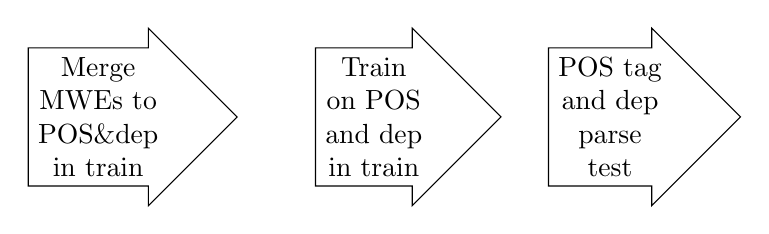
\begin{tikzpicture}[every node/.style={single arrow, draw, align=center}]
        \node  at (0.5,0) {Merge\\ MWEs to \\POS\&dep\\ in train};
        \node  at (4,0) {Train\\ on POS\\ and dep\\ in train};
        \node  at (7,0) {POS tag\\ and dep\\ parse\\ test};
\end{tikzpicture}
\vspace{2em}
\hspace{1em}
\framebox{\Longstack[c]{\textbf{Extract}\\ \textbf{MWE}\\ \textbf{tags and}\\ \textbf{labels}\\ \textbf{from test}}}
\caption{Steps of the USzeged system.}
\label{szeged}
\end{figure}

There are arguments for and against our approach. The system cannot handle multi-token MWEs where the elements are not connected in the tree and replacing the POS tags and dependency labels can have a negative effect on the accuracy of POS tagging\is{part-of-speech tagging} and parsing\is{parsing!dependency}. However, as our end goal is not the POS tagging\is{part-of-speech tagging} or dependency parse of the data, we believe that this side effect is negligible since higher-level applications (e.g.~machine translation) can profit from more accurate MWE identification. On the other hand, the approach has low technical requirements and it is very easily adaptable to other languages.


\subsection{Results}

We submitted the USzeged system for all languages in the shared task\is{PARSEME!shared task} with provided dependency analysis and POS tagging\is{part-of-speech tagging}. We attempted to use just the POS tagging component of our system on the languages that only had POS tagging\is{part-of-speech tagging} available to give partial results (i.e.~identifying only single-token MWEs), but we found that these languages incidentally had no or very few single-token MWEs (\ili{Farsi} 0, \ili{Maltese} 4, \ili{Romanian} 44, \ili{Slovene} 3, \ili{Turkish} 22), therefore we had no access to adequate training data and did not submit results for these languages.

Our results on the nine languages are reported in \cite{Simko2017}. Our system was submitted for \ili{German}, \ili{Greek}, \ili{Spanish}, \ili{French}, \ili{Hungarian}, \ili{Italian}, \ili{Polish}, \ili{Portuguese}, and \ili{Swedish}. For the evaluation, we employed the metrics used for the evaluation of the shared task \citep{MWEWorkshop}.


The F-scores show great differences between languages, but so did they for the other systems submitted.
Compared to the other, mostly closed-track systems, the USzeged system ranked close to or at the top on \ili{German}, \ili{Hungarian}, and \ili{Swedish}. For the other languages (except for \ili{Polish} and \ili{Portuguese}, where ours is the worst performing system), we ranked in the mid-range. 
%These results are related to the way our system works and the verbal MWE types frequent in the languages.

\subsection{Error analysis}

After receiving the gold annotation for the test corpora, we investigated the strengths and weaknesses of our system. 


Our error analysis showed that the USzeged system performs by far best on single-token MWEs, which in this dataset are mostly made up of the \isi{verb-particle construction} category, correctly identifying around 60\% of VPCs, but only about 40\% of other types on average. It is probably due to the fact that single-token MWEs are identified by POS tagging\is{part-of-speech tagging} techniques, which are known to obtain more accurate results in most languages than dependency parsing\is{parsing!dependency}.
%Verb-particle constructions are most likely to have a syntactic relationship between the MWE elements, which would support why our system is good at identifying them.

\ili{German}, \ili{Hungarian}, and \ili{Swedish} were also the languages with the highest proportions of the VPC type of verbal MWEs in the shared task, which also correlates with why our system performed best on them. Romance languages contain almost no VPCs and the remaining ones have much less also. In this way, the frequency of VPCs strongly influences our results on the given language.
%our achieved results seem to be dependent on the type of verbal MWEs frequent in that language because of the inherent characteristics of the system.

For \ili{French} and \ili{Italian}, our system also performed worse on IReflVs. In general, we had some trouble identifying longer IDs and LVCs and MWEs including prepositions. A further source of error was when there was no syntactic edge in between members of a specific MWE, for instance, in \ili{German}, the copula \textbf{sein} `be’ was often indirectly connected to the other words of the MWE (e.g.~\exlitidio{\lex{im Rennen sein}} {in race be} {to compete}), hence our method was not able to recognize it as part of the MWE. As our system does not restructure the syntactic trees, if the elements of a multi-token VMWE are not connected (i.e.~they do not form a graph) in their dependency annotation, we cannot identify the full MWE, however, we can still identify tokens of it correctly if at least two tokens within the MWE are attached.

\section{The extended system - USzeged+}

The primary aim of our extension was to be able to use our system for the languages in the shared task without any available POS and dependency data. We achieved this by parsing the annotated set in a preprocessing step. For the languages with gold POS and dependency data already available, we did not use this extra step (see \figref{szeged+}).

\begin{figure}
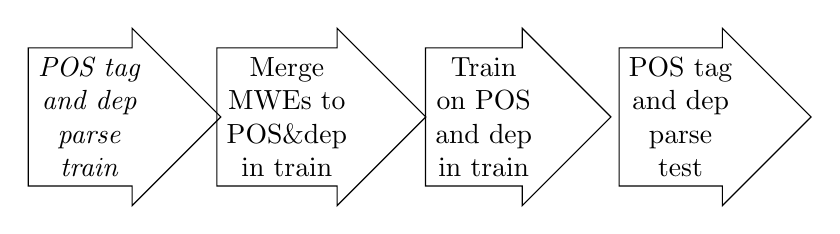
\begin{tikzpicture}[every node/.style={single arrow, draw, align=center}]
        \node {\textit{POS tag}\\ \textit{and dep}\\ \textit{parse}\\ \textit{train}};
        \node  at (2.5,0) {Merge\\ MWEs to \\POS\&dep\\ in train};
        \node  at (5,0) {Train\\ on POS\\ and dep\\ in train};
        \node  at (7.5,0) {POS tag\\ and dep\\ parse\\ test};
\end{tikzpicture}
\vspace{2em}
\framebox{\Longstack[c]{\textbf{Extract}\\ \textbf{MWE}\\ \textbf{tags and}\\ \textbf{labels}\\ \textbf{from test}}}
\caption{Steps of the USzeged+ system.}
\label{szeged+}
\end{figure}

We used data for the remaining languages from the \isi{Universal Dependencies} Project release 2.0 \citep{univdep} 
to train the Bohnet parser for POS-tagging and dependency parsing\is{parsing!dependency} and parsed the VMWE annotated shared task's training sets.
We should note that for some languages, the VMWE corpus and the \isi{Universal Dependencies} corpus are overlapping\is{verbal multiword expression!overlapping}. This influences our dependency parse to some degree as the training data might partially include the test data, but as our end goal here is not the full dependency parse of the texts (moreover, we already use gold dependency annotations for the languages which have it directly available), we feel that this factor is negligible. Henceforward, we exploited the very same processes as before: we merged the parsed data with the VMWE annotations and once again, trained the Bohnet parser on the VMWE merged data. We then parsed the test sets for the shared task and extracted the MWE POS-tagged and MWE dependency labeled words and phrases. 

\subsection{Results}

\tabref{resultstable2} shows the USzeged+ results for all shared task languages\is{PARSEME!shared task}. The languages covered by USzeged can be found in the upper part of the table, and the ones covered by USzeged+ are in the lower part. The ``upper'' languages of this table show differences to the results presented in \citep{Simko2017}. This is due to two main factors: the Bohnet parser was updated between our USzeged and USzeged+ versions of the system and we also corrected some bugs in our conversion tool. The basic working principles of our system are the same as described above.

\begin{table}
\centering
\caption{USzeged+ results: Languages covered by the previous system also are on top.}
\label{resultstable2}
\begin{tabular}{lllllll}
  \lsptoprule
& P-MWE & R-MWE  & F1-MWE  & P-token & R-token & F1-token \\
 \midrule
DE     & 31.16 & 40.20 & 35.11 & 40.65 & 43.05 & 41.82   \\
EL     & 37.01 & 30.20 & 33.26 & 49.14 & 32.65 & 39.23   \\
ES     & 25.67 & 52.00 & 34.37 & 32.13 & 55.20 & 40.62   \\
FR     & 31.23 & 31.60 & 31.41 & 43.57 & 39.44 & 41.40   \\
HU     & 62.02 & 71.34 & 66.36 & 58.45 & 69.08 & 63.32   \\
IT     & 9.21 & 6.80 & 7.83 & 33.29 & 18.70 & 23.94   \\
PL     & 35.96 & 59.40 & 44.80 & 41.33 & 63.68 & 50.13   \\
PT     & 33.29 & 52.80 & 40.84 & 40.76 & 58.96 & 48.20   \\
SV     & 14.96 & 22.88 & 18.09 & 20.55 & 28.21 & 23.77   \\
   \midrule 
BG     & 53.26 & 43.13 & 47.66 & 77.79 & 49.25 & 60.32   \\
CS     & 44.95 & 57.93 & 50.62 & 57.60 & 64.46 & 60.84   \\
FA     & 69.58 & 46.20 & 55.53 & 85.78 & 53.14 & 65.63   \\
HE     & 41.18 & 8.40 & 13.95 & 55.22 & 8.63 & 14.93  \\
LT     & 33.33 & 7.00 & 11.57 & 40.48 & 6.97 & 11.89  \\
MT     & 0.00 & 0.00 & 0.00 & 4.65 & 0.31 & 0.59  \\
RO     & 46.29 & 67.40 & 54.89 & 53.01 & 71.68 & 60.95  \\
SL     & 59.49 & 18.80 & 28.57 & 66.46 & 18.77 & 29.27  \\
TR     & 39.34 & 37.92 & 38.62 & 42.07 & 39.49 & 40.74  \\

  \lspbottomrule
\end{tabular}
\end{table}

Using gold or parsed POS and dependency data as the starting phase does not have a significant impact on the results (as we will show in another experiment in \sectref{goldorparsed}), with the exception of \ili{Maltese}. As \ili{Maltese} currently has no available \isi{Universal Dependencies} treebank, we used cross-language training to train our parser. As a Semitic language, \ili{Maltese} is basically related to Arabic but spelt with Latin characters and about half of its vocabulary originates from \ili{Italian}. Thus, we selected the available \ili{Italian} \isi{Universal Dependencies} treebank to train the parser and parse the VMWE train data. This had a very bad effect on our results: no full MWE could be correctly identified in the VMWE test set. Hence, for \ili{Maltese}, a more suitable solution is still to be found for our approach. For all other languages -- where the parser for the VMWE train data was trained on the same language -- the final results are much more comparable to those of the languages with gold trees.

Besides \ili{Maltese}, one of the languages where our system performed poorly is \ili{Italian}. We investigated the \ili{Italian} training corpus and found that its annotation has different underlying principles than most of the other corpora. Namely, it allows sentences to have multiple roots (which is prohibited in other dependency theories), hence it confuses the parser's training to a high degree and therefore very few valuable results (i.e.~MWE annotations) can be converted from the parsed sentences. Finally, \ili{Swedish} results are probably due to the small size of the training corpora.

\tabref{mwelevel} and \tabref{tokenlevel} show our results in F-score for the different MWE types; crossed out cells indicate that the type was not present for the given language. 

Overall, the USzeged+ system performs best on inherently reflexive verbs\is{inherently reflexive verb} (IReflV). IReflVs contain irreflexive pronouns, which show little variability\is{idiomatic variation}, thus they can be relatively easily recognized by the system. However, the system performs worst on idioms and the ``other'' category due to their bigger variability and the longer MWEs in these types. Light-verb constructions\is{light-verb construction} and verb-particle constructions\is{verb-particle construction} show varied results depending on the variability of the category in the given language. VPCs could be easily recognized in \ili{Hungarian} (an F-score over 80), while LVC identification was most successful in \ili{Romanian} (an F-score of 70).

There are also differences in the annotations of the languages: for instance, \ili{Farsi} contains only VMWEs for the ``other'' category, which makes it hard to make any comparisons with the other languages on the effective identification of VMWE categories.

The results also show that while our system has very similar average results on the other language group of the shared task (interestingly even the ``other'' category, which is probably due to \ili{Farsi}), results are much lower on Romance languages on average. This is most probably due to the issues on the \ili{Italian} dependency data (see above), which resulted in poor performance for almost all of the VMWE categories in \ili{Italian}.


\begin{table}
\centering
\caption{USzeged+ MWE-level F-score results for the different MWE types.}
\label{mwelevel}
\begin{tabular}{lllllll}
  \lsptoprule
 & all   & VPC    & LVC    & ID     & IReflV & OTH    \\
 \midrule
BG  & 47.66 &  -       & 20.44 & 18.79 & 60.70 &  -   \\
CS  & 50.62 &  -       & 26.96 & 2.51 & 61.71 & 0.00\\
DE  & 35.11 & 54.55 & 10.39 & 16.16 & 17.50 &  -   \\
EL  & 33.26 & 56.00 & 36.68 & 9.52 &  -       & 8.00\\
ES  & 34.37 &  -       & 32.40 & 9.70 & 43.04 & 0.00\\
FA  & 55.53 &  -       &  -       &  -       &  -       & 55.53 \\
FR  & 31.41 &  -       & 27.67 & 16.48 & 52.94 & 0.00\\
HE  & 13.95 & 9.35 & 24.20 & 0.00 &  -       & 13.76 \\
HU  & 66.36 & 80.59 & 35.47 &  -       &  -       &  -   \\
IT  & 7.83 & 22.22 & 5.13 & 5.05 & 0.00 & 0.00\\
LT  & 11.57 &  -       & 23.53 & 0.00 &  -       &  -   \\
MT  & 0.00 &  -       & 0.00 & 0.00 &  -       & 0.00\\
PL  & 44.80 &  -       & 25.38 & 0.00 & 65.63 &  -   \\
PT  & 40.84 &  -       & 45.89 & 11.57 & 40.99 &  -   \\
RO  & 54.89 &  -       & 70.59 & 20.51 & 54.92 &  -   \\
SL  & 28.57 & 0.00 & 14.29 & 1.90 & 45.71 & 0.00\\
SV  & 18.09 & 22.11 & 8.70 & 0.00 & 2.90 & 0.00\\
TR  & 38.62 &  -       & 39.77 & 32.71 &  -       & 34.34 \\
 \midrule
Average  & 34.08 & 34.97 & 26.32 & 9.06 & 40.54 & 10.15 \\


  \lspbottomrule
\end{tabular}
\end{table}


\begin{table}
\centering
\caption{USzeged+ system's token-level F-score results for the different MWE types.}
\label{tokenlevel}
\begin{tabular}{lllllll}
  \lsptoprule
  & all   & VPC    & LVC    & ID     & IReflV & OTH    \\
 \midrule
BG  & 60.32 &  -       & 32.63 & 24.30 & 74.05 &  -     \\
CS  & 60.84 &  -       & 31.78 & 17.87 & 72.44 & 0.00\\
DE  & 41.82 & 56.14 & 12.58 & 32.41 & 24.85 &  -     \\
EL  & 39.23 & 56.00 & 40.65 & 19.97 &  -       & 4.04\\
ES  & 40.62 &  -       & 35.86 & 22.47 & 44.27 & 0.00\\
FA  & 65.63 &  -       &  -       &  -       &  -       & 65.63\\
FR  & 41.40 &  -       & 30.17 & 36.11 & 52.94 & 0.00\\
HE  & 14.93 & 13.82 & 23.21 & 10.62 &  -       & 10.83\\
HU  & 63.32 & 80.59 & 40.82 &  -       &  -       &  -     \\
IT  & 23.94 & 27.78 & 12.60 & 23.78 & 0.00 & 0.00\\
LT  & 11.89 &  -       & 23.30 & 3.28 &  -       &  -     \\
MT  & 0.59 &  -       & 0.71 & 0.33 &  -       & 0.00\\
PL  & 50.13 &  -       & 28.18 & 13.19 & 69.44 &  -     \\
PT  & 48.20 &  -       & 50.73 & 27.80 & 42.07 &  -     \\
RO  & 60.95 &  -       & 73.03 & 48.88 & 55.75 &  -     \\
SL  & 29.27 & 1.70 & 15.87 & 9.36 & 46.29 & 0.00\\
SV  & 23.77 & 26.80 & 8.79 & 2.26 & 2.90 & 0.00\\
TR  & 40.74 &  -       & 41.32 & 34.43 &  -       & 36.36\\
\midrule
Average  & 39.87 & 37.55 & 29.54 & 20.44 & 44.09 & 10.62\\



  \lspbottomrule
\end{tabular}
\end{table}

We did some error analysis based on the languages we can speak. This revealed that as for LVCs, our system usually marks as false positives those verb-object pairs where the verb is an otherwise frequent light verb in the given language (e.g. (PT) \nltliidio{\lex{ter}}{to have}). Also, participle forms of LVCs were often missed in (FR) \nltliidio{\lex{études menées}}{studies conducted}. As for VPCs, many compositional instances of verbs with particles were falsely marked in \ili{German} and in \ili{Hungarian}, like (DE) \nltliidio{\lex{anheben}} {hang up}. The same is true for IReflVs: compositional ones like (PT) \nltliidio{\lex{encantar-se}}{enchant} were sometimes falsely identified as VMWEs. A further source of errors could also be some inconsistencies in the data: in a few cases, annotators missed to mark some clear examples of VMWEs in the test data, which resulted again in false positives. Finally, the \ili{German} corpus contained some \ili{English} sentences, e.g.~\textit{[...] if Proporz were to be taken out of the Austrian economy, actual unemployment would be ... higher?} In this sentence, \textit{be} and \textit{higher} are marked as an instance of VPC. The word \textit{be} is a typical particle in \ili{German}, while last words of the sentences are often verbs in \ili{German} due to word order reasons. Probably this is the reason why the system gave this analysis.

As our system uses different methods to assign single- and multi-token MWE labels, we also investigated our results for these separately. We found that most languages only contain no or very few single-token MWEs, with the exception of \ili{German} and \ili{Hungarian}. Approximately 12\% of VMWEs are single-token in the \ili{German} data, while they make up of 40\% of VMWEs in the \ili{Hungarian} data. \tabref{singletokenresults} shows our system's accuracy on single- and multi-token MWEs for \ili{German} and \ili{Hungarian}.

\begin{table}
\centering
\caption{Accuracy on single- and multi-token MWEs for German and Hungarian.}
\label{singletokenresults}
\begin{tabular}{lllllll}
  \lsptoprule
  & single-token & multi-token & overall  \\
 \midrule
 DE  & 64 & 36 & 46   \\
HU  & 83  & 43.3 & 68.9 \\
  \lspbottomrule
\end{tabular}
\end{table}

These results confirm that our system achieves better results on single-token MWEs than on multi-token ones.

\section{Gold or parsed?}
\label{goldorparsed}

In this last section, we describe a small experiment comparing our new addition to the system: the parsed POS and dependency data. We compare our results on \ili{Hungarian} using the gold POS and dependency data with an experimental setup mirroring that of the languages without this gold data. We used the \ili{Hungarian} \isi{Universal Dependencies} treebank to train the Bohnet parser for POS tagging\is{part-of-speech tagging} and dependency parsing\is{parsing!dependency} and exploited these trained models to parse the VMWE train sentences. 

\tabref{goldvsparsed} shows the results of this experiment; the results for HU-GOLD are the same as the ones for \ili{Hungarian} in the above tables. The results show that gold and parsed methods in our system can provide very comparable results. Interestingly, in both MWE-level and token-level results, the parsed method provides much higher precision but lower recall than the gold method. 

For MWE types, LVCs are causing the main difference in the two systems. Many VPCs in the \ili{Hungarian} data are single-token, so our system deals with them on the level of POS tagging\is{part-of-speech tagging}, which is not affected by gold or parsed dependency trees.

Overall, both options achieved approximately the same results in the automatic VMWE recognition task.

\begin{table}
\centering
\caption{Gold and parsed results for Hungarian.}
\label{goldvsparsed}
\begin{tabular}{lll}
  \lsptoprule
& HU-GOLD        & HU-PARSED \\
 \midrule
P-MWE      & 62.02 & 74.94\\
R-MWE      & 71.34 & 62.93\\
F-MWE      & 66.36 & 68.41\\
\midrule
P-token    & 58.45 & 74.74\\
R-token    & 69.08 & 53.85\\
F-token    & 63.32 & 62.60\\
\midrule 
F-VPC-MWE    & 80.59 & 78.59\\
F-LVC-MWE    & 35.47 & 25.41\\
\midrule 
F-VPC-token  & 79.05 & 77.66\\
F-LVC-token  & 40.82 & 25.71\\

  \lspbottomrule
\end{tabular}
\end{table}

\section{Conclusions}

In our chapter, we presented our system for verbal MWE recognition. The system uses POS tagging and dependency parsing as a means of finding verbal MWEs in multiple languages.

Apart from parsing-based solutions (\cite{W17-1717}, \cite{W17-1706} and our system), the shared task hosted a number of other approaches, like neural networks (\cite{W17-1707}) or sequence labeling based models (\cite{borocs2017}, \cite{maldonado2017}). In the final results, parsing-based systems achieved the best results for almost all languages, showing that this approach works very well for language independent MWE identification.

Our chapter further shows that it is possible to build a highly language independent MWE detection methodology that makes use of a limited amount of language-specific data and achieve reasonable results. 

\section*{Acknowledgements}

We would like to thank the anonymous reviewers and the volume editors for their invaluable comments on our work.

Veronika Vincze was supported by the UNKP-17-4 New National Excellence Program of the Ministry of Human Capacities, Hungary.

\section*{Abbreviations}
\begin{tabularx}{.48\textwidth}{ll}
\textsc{id} & idiom\\
\textsc{IReflV} & inherently reflexive verb \\
\textsc{lvc} & light-verb construction \\
\textsc{mwe} & multiword expression \\
\end{tabularx}
\begin{tabularx}{.48\textwidth}{ll}
\textsc{oth} & other  \\
\textsc{pos} & part of speech  \\
\textsc{vpc} & verb-particle construction \\
\textsc{vmwe} & verbal multiword expression \\
\end{tabularx}



{\sloppy
\printbibliography[heading=subbibliography,notkeyword=this]
}
\end{document}
